\begin{center}
    \vspace*{1.5cm}
    {\fontsize{20}{20}\textbf{Vinvisor}}\\
    \vspace{0.7cm}
    {\fontsize{12}{12}\textit{Om den vita skjortan själv får välja}}
\end{center}
\addtocwithheader{Vinvisor}  % Add entry to TOC and set header\noBackground
\noBackground

\newpage
\noBackground

\begin{textblock*}{3cm}(4.1cm,7.3cm) % {width}(x, y)
    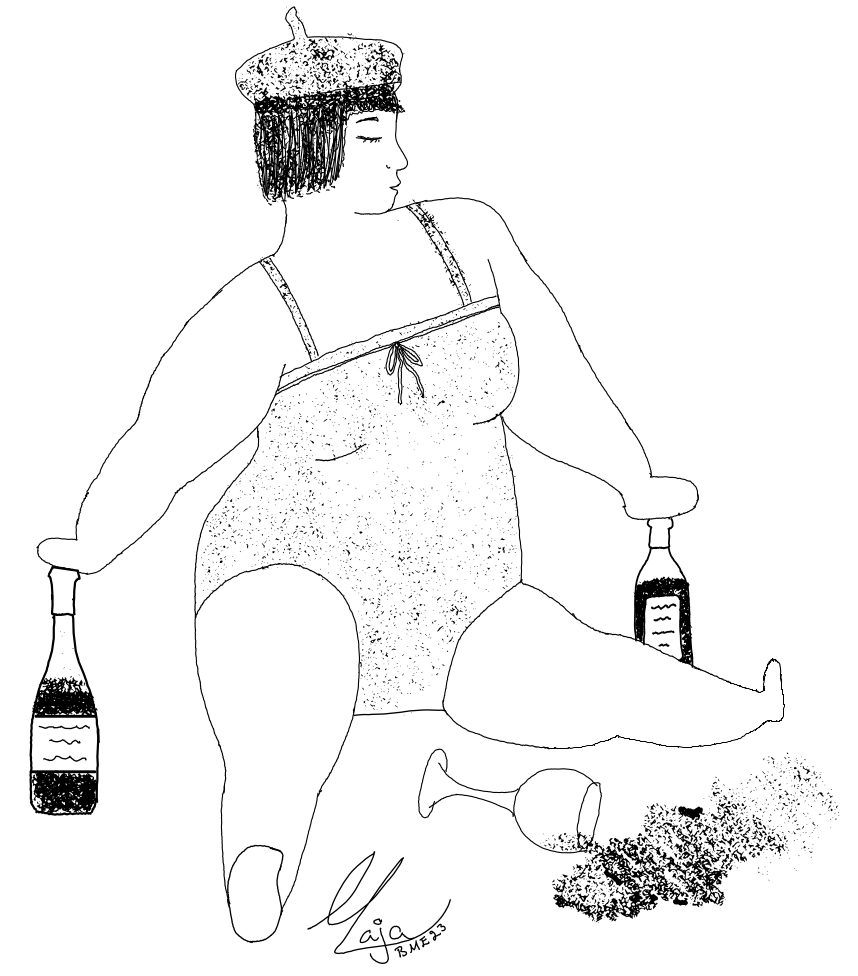
\includegraphics[width=6cm]{./bilder/majas-bilder/feta_fransyskor.png}
\end{textblock*}


\subsection*{Feta fransyskor} 
\index[alfa]{Feta fransyskor}
\index[anfa]{Feta fransyskor}
\songinfo{Mel: Militärmarsch av Schubert\\
K-sektionen Sångarstriden 1985}

\begin{parse lines}[\noindent]{#1\\}
    Feta fransyskor som svettas om fötterna,
    de trampar druvor
    som sedan ska jäsas till vin
    Transpirationen viktig é,
    ty den ge'
    fin bouquet
    Vårtor och svampar följer me'
    men vad gör väl de'?

    För vi vill ha vin,
    vill ha vin,
    vill ha mera vin,
    även om följderna blir
    att vi må lida pin
    Flaskan och glaset gått i sin
    Hit med vin, mera vin!
    Tror ni att vi är fyllesvin?
    {\Large Ja!} (Fast större!)
\end{parse lines}


\newpage
\resetBackground

\subsection*{Imsig vimsig} 
\index[alfa]{Imsig vimsig}
\index[anfa]{Imsig vimsig blir man}
\songinfo{Mel: Imse vimse spindel}

\begin{parse lines}[\noindent]{#1\\}
    Åsnan dricker vatten, det gör inte vi
    Vi dricker bara sådant folk har trampat i
    Kamelen uti öknen söker en oas
    Det gör inte vi, vi har vin i våra glas

    Imsig vimsig blir man, utav lite vin
    Kliver upp på stolen, verkar piggelin
    Ramlar under bordet, sussar en minut
    Vaknar av att vinet i glaset tagit slut

\end{parse lines}


\subsection*{Korkskruvens visa} 
\index[alfa]{Korkskruvens visa}
\index[anfa]{Nu har vi rus}
\songinfo{Mel: Nu har vi ljus}

\begin{parse lines}[\noindent]{#1\\}
    Nu har vi rus här i vårt hus
    Korken är borta hopp tralalala
    Doften är ljuv, jag är en skruv,
    jag är en skruv
    Jag kan inte öppna bag-in-boxen
    Jag kan inte öppna bag-in-boxen
    Lalala lalalalala 
    lalalalala lala lala
\end{parse lines}

\vissteduatt{Visste du att radioentusiaster från ETF lader grunden till det \\som idag är Radio AF?}

\newpage


\subsection*{Lyft ditt välförsedda glas} 
\index[alfa]{Lyft ditt välförsedda glas}
\index[anfa]{Lyft ditt välförsedda glas}
\songinfo{Mel: Ding dong merrily on high}

\begin{parse lines}[\noindent]{#1\\}
    Lyft ditt välförsedda glas
    Det är en härlig börda
    Nu har grabbarna kalas
    Ve segern snart skall skörda
    ||: Ding dingedingeding dingedingeding
    dingedingeding dong dong
    Imorgon är det lördag :||

    Sätt nu glaset till din mun
    Se döden på dig väntar
    Nu har grabbarna kalas
    Hör liemannen flämtar
    ||: Ding dingedingeding dingedingeding
    dingedingeding dong dong
    Begravningsklockor klämtar :||

\end{parse lines}

\newpage

\hspace{1cm}
\subsection*{Bordeaux, bordeaux} 
\index[alfa]{Bordeaux, bordeaux}
\index[anfa]{Jag minns än idag hur min fader}
\songinfo{Mel: I sommarens soliga dagar}

\begin{parse lines}[\noindent]{#1\\}
    Jag minns än idag hur min fader
    kom hem ifrån staden så glader
    och rada' upp flaskor i rader
    och sade nöjd som så:
    "Bordeaux, Bordeaux!"

    Han drack ett glas, kom i extas,
    och sedan blev det stort kalas
    Och vi små glin, ja vi drack vin
    som första klassens fyllesvin
    Och vi dansade runt där på borden
    och skrek så vi blev blå:
    "Bordeaux, Bordeaux!"


\end{parse lines}

\subsection*{Vinbröder} 
\index[alfa]{Vinbröder}
\index[anfa]{Två bröder, Jan-Ove och Hadar}
\songinfo{Mel: I sommarens soliga dagar}

\begin{parse lines}[\noindent]{#1\\}
    Två bröder, Jan-Ove och Hadar,
    de plockade fram sina spadar,
    och grävde en grop bakom huset.
    De hade en idé:
    Vadå, vadå?
    


    Jo, priset på, Kir och Bordeaux,
    är högt men om man gjorde så,
    att man i gropen lade ner,
    två kilo jäst och en back MER,
    så skulle det nog vara möjligt
    att producera vin i detta hål!


\end{parse lines}


\subsection*{Karnaugh, karnaugh} 
\index[alfa]{Karnaugh, karnaugh}
\index[anfa]{Karnaugh, karnaugh}
\songinfo{Mel: I sommarens soliga dagar}

\begin{parse lines}[\noindent]{#1\\}
    Jag minns än i dag hur min fader
    kom hem i från labbet så glader
    och rada' upp bitar i rader
    och sade glad som så:
    Karnaugh, Karnaugh!

    Å ett å noll \& noll å ett 
    å booleska uttryck det är fett!
    Med ett å noll \& noll å ett,
    ska du nu se att det blir rätt,
    Men vi felsökte våra signaler,
    och det blev fel ändå
    Karnaugh, Karnaugh!
\end{parse lines}


\newpage


\subsection*{I sommarens soliga dagar} 
\index[alfa]{I sommarens soliga dagar}
\index[anfa]{I sommarens soliga dagar}
\songinfo{Mel: I sommarens soliga dagar\\
Text: Anders Nilsson $\pi$03 och Björn Carlin $\pi$02}

\begin{parse lines}[\noindent]{#1\\}
    I sommarens soliga dagar
    Kall rå fisk till alla vi lagar
    Och sätter oss ute i hagar
    Där maten härsken står
    Bakteriehärd av solen närd

    Den höjer högt sitt blanka svärd
    Men mot dess hot vi funnit bot 
    Vi sätter spritens krafter mot
    För spriten kan döda det mesta
    Vi hälsan återfår, Gutår! Gutår!
\end{parse lines}

\vissteduatt{Visste du att LTH-fontänen invigdes 1970 men plockades ner 1996
\\efter otaliga försök att reparera den? Kvar står stålskelettet.}

\newpage
\noBackground

\begin{textblock*}{3cm}(5cm,8cm) % {width}(x, y)
    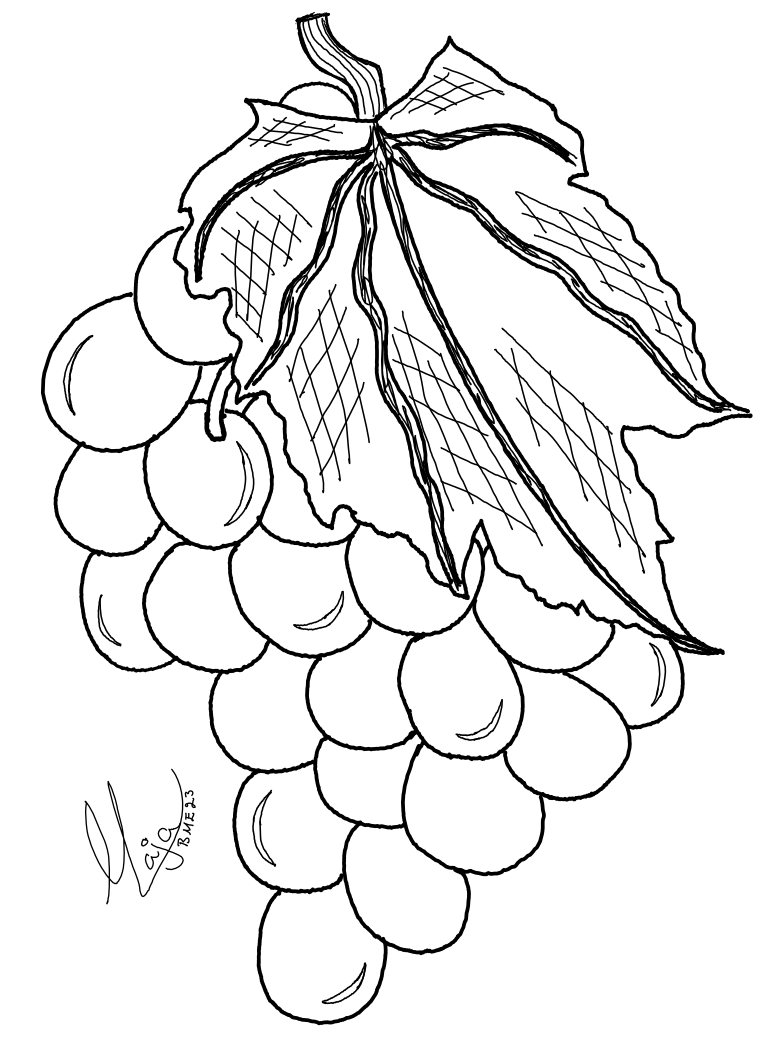
\includegraphics[width=4cm]{./bilder/majas-bilder/vindruvor.png}
\end{textblock*}



\subsection*{Magnumflaskan Åkesson} 
\index[alfa]{Magnumflaskan Åkesson}
\index[anfa]{Magnumflaskan Åkesson}
\songinfo{Mel: Teddybjörnen Fredriksson\\
Lundakarnevalen 2010}

\begin{parse lines}[\noindent]{#1\\}
    För längesen, när jag fyllde 15 år
    fick jag en flaska av min mor
    Hon sa "Mitt barn, dela den med vännerna
    För den är faktiskt ganska stor."

    Magnumflaskan Åkesson,
    du var så stor och tung
    Jag gick runt med dig i hand,
    och i Dalby var jag kung

    Magnumflaskan Åkesson,
    din kork försvann i skyn
    Men jag drack dig bara själv
    Och kräktes i hela byn
\end{parse lines}


\newpage
\resetBackground

\subsection*{Detta är jag} 
\index[alfa]{Detta är jag}
\index[anfa]{Jag är en enkel mytoman}
\songinfo{Mel: Med en enkel tulipan\\
Lundakarnevalen 2018}

\begin{parse lines}[\noindent]{#1\\}
    Jag är en enkel mytoman
    Som utav ren slentrian
    Han ljugit till mig en plats vid bordet
    och ett glas rödvin    
    
\end{parse lines}

\subsection*{Kosmetisk visa} 
\index[alfa]{Kosmetisk visa}
\index[anfa]{Du behöver inte ha nåt läppstift alls}
\songinfo{Mel: She’ll be Coming ‘Round the Mountain\\
Lundakarnevalen 2002}

\begin{parse lines}[\noindent]{#1\\}
    Du behöver inte ha nåt läppstift alls,
    du behöver inte ha nåt läppstift alls,
    för när vinet börjar flöda,
    färgas läpparna ju röda,
    liksom tungan, hakan, skjortan och din hals!
\end{parse lines}



\newpage
\noBackground


\begin{textblock*}{3cm}(5.8cm,3.8cm) % {width}(x, y)
    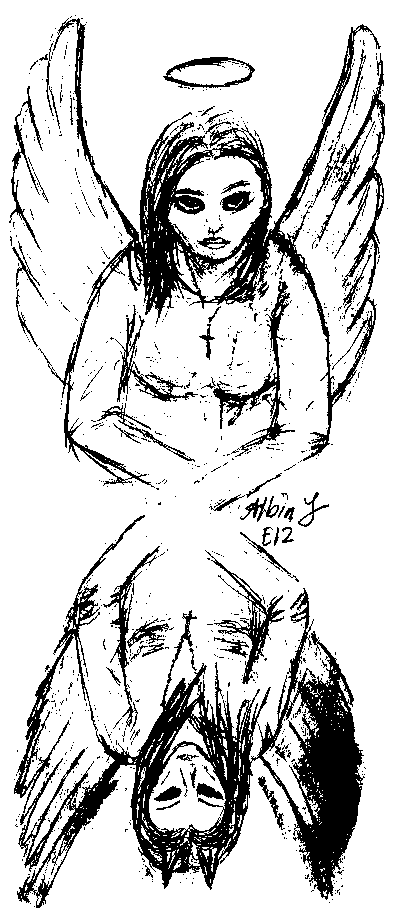
\includegraphics[width=4.0cm]{./bilder/dance_macabre_transparent.png}
\end{textblock*}

\subsection*{Dance macabre} 
\index[alfa]{Dance macabre}
\index[anfa]{runt våran stuga, små djävlar sluga}
\songinfo{Mel: Vårvindar friska}

\begin{parse lines}[\noindent]{#1\\}
    Runt våran stuga, små djävlar sluga
    tassa så tyst med bockfot och svans
    Varulvar yla, isande kyla
    sveper i dimman, fantygets dans
    Bäva, o broder, lyssna och hör
    vrålen från gast, som osalig dör
    Satan han skrattar,
    flaskan han fattar,
    super tills dagen gryr.

    Gastar och spöken
    skymta i köken,
    dödingar släpa ruttnande lik
    Benrangel skramla,
    spökhänder famla,
    kväva din strupes rosslande skrik
    Helvetes alla fasor släpps loss
    Fan rider här med hela sin tross
    Göm dig i stugan,
    du har fått flugan
    Dille det blir din lott

\end{parse lines}

\vissteduatt{Visste du att man viskar hela låten fram till "Helvetets alla fasor..." 
\\då tar man i för Kung och fosterland?}


\newpage
